%!TEX program = xelatex
\documentclass[dvipsnames, svgnames,a4paper,11pt]{article}
% ----------------------------------------------------- 
%	加边框的命令
%	参考:https://tex.stackexchange.com/questions/531559/how-to-add-the-page-border-for-first-two-pages-in-latex
\usepackage{tikz}
\usetikzlibrary{calc}
\usepackage{eso-pic}
\AddToShipoutPictureBG{%
\begin{tikzpicture}[overlay,remember picture]
\draw[line width=0.6pt] % 边框粗细
    ($ (current page.north west) + (0.6cm,-0.6cm) $)
    rectangle
    ($ (current page.south east) + (-0.6cm,0.6cm) $); % 边框位置
\end{tikzpicture}}


\usepackage{xcolor}
\definecolor{c1}{HTML}{086173} % 目录颜色 原版为2752C9 紫灰色535AAA 蓝紫色0B0DB7 深蓝色070F94 湖绿色219394 松石灰绿086173
\definecolor{c2}{HTML}{E20129} % 引用颜色 原版\definecolor{c2}{RGB}{190,20,83} 橙色F24729

\usepackage{ctex}
\usepackage[top=28mm,bottom=28mm,left=15mm,right=15mm]{geometry}
\usepackage{hyperref} 
\hypersetup{
	colorlinks,
	linktoc = section, % 超链接位置,选项有section, page, all
	linkcolor = c1, % linkcolor 目录颜色
	citecolor = c1  % citecolor 引用颜色
}
\usepackage{amsmath,enumerate,multirow,float}
\usepackage{tabularx}
\usepackage{tabu}
\usepackage{subfig}
\usepackage{fancyhdr}
\usepackage{graphicx}
\usepackage{wrapfig}  
\usepackage{physics}
\usepackage{appendix}
\usepackage{amsfonts}

%
\usepackage{tcolorbox}
\tcbuselibrary{skins,breakable}
\newtcolorbox{tbox}[2][]{
    colframe=black!70!,
    breakable,
    enhanced,
	boxrule =0.5pt,
    title = {#2},
    fonttitle = \large\kaishu\bfseries,
	drop fuzzy shadow,
    #1
}
\newtcolorbox[auto counter,number within=section]{question}[1][]{
  top=2pt,bottom=2pt,arc=1mm,
  boxrule=0.5pt,
%   frame hidden,
  breakable,
  enhanced, %跨页后不会显示下边框
  coltitle=c1!80!gray,
  colframe=c1,
  colback=c1!3!white,
  drop fuzzy shadow,
  title={思考题~\thetcbcounter:\quad},
  fonttitle=\bfseries,
  attach title to upper,
  #1
}

% ---------------------------------------------------------------------
%	利用cleveref改变引用格式,\cref是引用命令
\usepackage{cleveref}
\crefformat{figure}{#2{\textcolor{c2}{Figure #1}}#3} % 图片的引用格式
\crefformat{equation}{#2{(\textcolor{c2}{#1})}#3} % 公式的引用格式
\crefformat{table}{#2{\textcolor{c2}{Table #1}}#3} % 表格的引用格式


% ---------------------------------------------------------------------
%	页眉页脚设置
\fancypagestyle{plain}{\pagestyle{fancy}}
\pagestyle{fancy}
\lhead{\kaishu 中山大学物理与天文学院电子技术实验\uppercase\expandafter{\romannumeral1}} % 左边页眉,学院 + 课程
\rhead{\kaishu 实验报告By黄罗琳} % 右边页眉,实验报告标题
\cfoot{\thepage} % 页脚,中间添加页码


% ---------------------------------------------------------------------
%	对目录、章节标题的设置
\renewcommand{\contentsname}{\centerline{\huge 目录}}
\usepackage{titlesec}
\usepackage{titletoc}
% \titleformat{章节}[形状]{格式}{标题序号}{序号与标题间距}{标题前命令}[标题后命令]
\titleformat{\section}{\centering\LARGE\songti}{}{1em}{}

% ---------------------------------------------------------------------
%   listing代码环境设置
\usepackage{listings}
\lstloadlanguages{python}
\lstdefinestyle{pythonstyle}{
backgroundcolor=\color{gray!5},
language=python,
frameround=tftt,
frame=shadowbox, 
keepspaces=true,
breaklines,
columns=spaceflexible,                   
basicstyle=\ttfamily\small, % 基本文本设置,字体为teletype,大小为scriptsize
keywordstyle=[1]\color{c1}\bfseries, 
keywordstyle=[2]\color{Red!70!black},   
stringstyle=\color{Purple},       
showstringspaces=false,
commentstyle=\ttfamily\scriptsize\color{green!40!black},%注释文本设置,字体为sf,大小为smaller
tabsize=2,
morekeywords={as},
morekeywords=[2]{np, plt, sp},
numbers=left, % 代码行数
numberstyle=\it\tiny\color{gray}, % 代码行数的数字字体设置
stepnumber=1,
rulesepcolor=\color{gray!30!white}
}




% ---------------------------------------------------------------------
%	其他设置
\def\degree{${}^{\circ}$} % 角度
\graphicspath{{./images/}} % 插入图片的相对路径
\allowdisplaybreaks[4]  %允许公式跨页 
\usepackage{lipsum}
\usepackage{adjustbox}
\usepackage{multirow}

%\usepackage{mathrsfs} % 字体
%\captionsetup[figure]{name=Figure} % 图片形式
%\captionsetup[table]{name=Table} % 表格形式
\begin{document}
	
	% 实验报告封面	
	% 顶栏
	\begin{table}
		\renewcommand\arraystretch{1.7}
		\begin{tabularx}{\textwidth}{
				|X|X|X|X
				|X|X|X|X|}
			\hline
			\multicolumn{2}{|c|}{预习报告}&\multicolumn{2}{|c|}{实验记录}&\multicolumn{2}{|c|}{分析讨论}&\multicolumn{2}{|c|}{总成绩}\\
			\hline
			\LARGE25 & & \LARGE25 & & \LARGE30 & & \LARGE80 & \\
			\hline
		\end{tabularx}
	\end{table}
	% ---
	
	% 信息栏
	\begin{table}
		\renewcommand\arraystretch{1.7}
		\begin{tabularx}{\textwidth}{|X|X|X|X|}
			\hline
			年级、专业: & 2022级 物理学 &组号: &D8 \\
			\hline
			姓名: &  黄罗琳  & 学号: &22344001   \\
			\hline
			实验时间: & 2024/5/8 & 教师签名: & \\
			\hline
		\end{tabularx}
	\end{table}
	% ---
	
	% 大标题
	\begin{center}
		\LARGE ET9、ET10 \quad 两级阻容耦合放大电路、负反馈放大电路 
		
	\end{center}
	% ---
	
	% 注意事项
	
	% 基本
	\textbf{【实验报告注意事项】}
	\begin{enumerate}
		\item 实验报告由三部分组成:
		\begin{enumerate}
			\item 预习报告:课前认真研读实验讲义,弄清实验原理;实验所需的仪器设备、用具及其使用、完成课前预习思考题;了解实验需要测量的物理量,并根据要求提前准备实验记录表格(可以参考实验报告模板,可以打印)。\textcolor{red}{\textbf{(20分)}}
			\item 实验记录:认真、客观记录实验条件、实验过程中的现象以及数据。实验记录请用珠笔或者钢笔书写并签名(\textcolor{red}{\textbf{用铅笔记录的被认为无效}})。\textcolor{red}{\textbf{保持原始记录,包括写错删除部分,如因误记需要修改记录,必须按规范修改。}}(不得输入电脑打印,但可扫描手记后打印扫描件);离开前请实验教师检查记录并签名。\textcolor{red}{\textbf{(30分)}}
			\item 数据处理及分析讨论:处理实验原始数据(学习仪器使用类型的实验除外),对数据的可靠性和合理性进行分析;按规范呈现数据和结果(图、表),包括数据、图表按顺序编号及其引用;分析物理现象(含回答实验思考题,写出问题思考过程,必要时按规范引用数据);最后得出结论。\textcolor{red}{\textbf{(30分)}}
		\end{enumerate}
		\textbf{实验报告就是将预习报告、实验记录、和数据处理与分析合起来,加上本页封面。\textcolor{red}{(80分)}}
		\item 每次完成实验后的一周内交\textbf{实验报告}(特殊情况不能超过两周)。
		
	\end{enumerate}
	

	

	\clearpage
	\tableofcontents
	\clearpage
	% ---
	
	
	
	% 预习报告	
	
	% 小标题
	\setcounter{section}{0}
	\section{ET9 两级阻容耦合放大电路 \quad\heiti 预习报告}
	% ---
	
	% 实验目的
	\subsection{实验目的}
	\begin{enumerate}
		\item 掌握两级阻容耦合放大电路静态工作点的调整方法。
		\item 掌握两级阻容耦合放大电路电压放大倍数的测量方法。
		\item 掌握放大电路频率特性的测定方法。
		
	\end{enumerate}
	% ---
	
	% 仪器用具
	\subsection{仪器用具}
	\begin{table}[htbp]
		\centering
		\renewcommand\arraystretch{1.6}
		% \setlength{\tabcolsep}{10mm}
		\begin{tabular}{p{0.05\textwidth}|p{0.20\textwidth}|p{0.05\textwidth}|p{0.5\textwidth}}
			\hline
			编号 & 仪器用具名称 & 数量 & 主要参数(型号,测量范围,测量精度等) \\
\hline
1 & 实验电路板 & 1 &  \\
2 & 数字万用表 & 1 & RIGOL DM3058E \\
3 & 函数信号发生器 & 1 & RIGOL DG4162 \\
4 & 双踪示波器 & 1 & RIGOL DS1104Z PLUS \\
5 & 直流稳压电源 & 1 & RIGOL DP831 \\
6 & 导线 & 若干 & 无 \\
			\hline
		\end{tabular}
	\end{table}
	% ---
	
	% 原理概述
	\subsection{原理概述}
	
多级放大电路是一种用于提高电压增益的电路。阻容耦合放大器是多级放大电路中最常见的形式,其特征在于各级直流工作点互不影响,可以独立调整。多级放大电路中的前一级输出电压作为后一级的输入电压,因此总电压放大倍数为各级放大倍数的乘积:

\[
\dot{A}_u = \dot{A}_{u1} \cdot \dot{A}_{u2} \ldots \cdot \dot{A}_{un}.
\]

由于阻容耦合电路中的电抗性元件,放大倍数随信号频率的变化而改变,频率响应在高、低频段会出现降低的情况。
\begin{figure}[{H}]
	\centering
	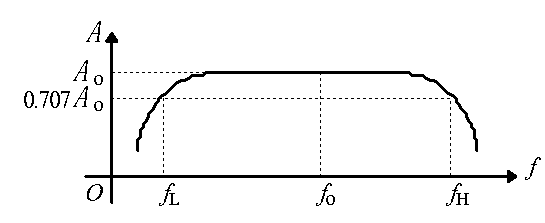
\includegraphics[width=0.5\linewidth]{原理.png
	}
	
	\label{}
\end{figure}

多级放大电路的上限频率 \(f_H\) 表示电路能够处理的最高频率。对于多级电路,其上限频率可以通过以下近似公式计算:

\[
\frac{1}{f_H} \approx 1.1 \sqrt{\frac{1}{f_{H1}^2} + \frac{1}{f_{H2}^2} + \ldots + \frac{1}{f_{Hn}^2}}.
\]

这个公式表明,上限频率与各级上限频率的平方和取倒数,然后取平方根有关。较低的上限频率会对整个电路的上限频率产生更大的影响。

多级放大电路的下限频率 \(f_L\) 是电路能够处理的最低频率。下限频率与各级下限频率的平方和取平方根有关,公式如下:

\[
f_L \approx 1.1 \sqrt{f_{L1}^2 + f_{L2}^2 + \ldots + f_{Ln}^2}.
\]

较高的下限频率会影响整个电路的最低频率。这个公式表明,下限频率取决于各级的下限频率,且最重要的一级是下限频率最高的那一级。

在实际的多级放大电路中,当各放大级的时间常数相差悬殊时,可取起主要作用的那一级作为估算的依据。例如,若其中第 $k$ 级的上限频率 $f_{Hk}$比其他各级小得多时,可近似认为总的 $f_H=f_{HK}$。同理,若其中第$m$级的下限频率${f}_{Lm}$比其他各级大得多时,可以近似认为总的 $f_{L}={f}_{Lm}$。

	\clearpage
	\section{ET10 负反馈放大电路  \quad\heiti 预习报告}
	
	\subsection{实验目的}
	\begin{enumerate}
		\item 熟悉负反馈放大电路性能指标的测试方法。
		\item 通过实验深入理解负反馈对放大电路性能的影响。
		
		
	\end{enumerate}
	% ---
	
	% 仪器用具
	\subsection{仪器用具}
	\begin{table}[htbp]
		\centering
		\renewcommand\arraystretch{1.6}
		% \setlength{\tabcolsep}{10mm}
		\begin{tabular}{p{0.05\textwidth}|p{0.20\textwidth}|p{0.05\textwidth}|p{0.5\textwidth}}
			\hline
			编号 & 仪器用具名称 & 数量 & 主要参数(型号,测量范围,测量精度等) \\
\hline
1 & 实验电路板 & 1 &  \\
2 & 数字万用表 & 1 & RIGOL DM3058E \\
3 & 函数信号发生器 & 1 & RIGOL DG4162 \\
4 & 双踪示波器 & 1 & RIGOL DS1104Z PLUS \\
5 & 直流稳压电源 & 1 & RIGOL DP831 \\
6 & 导线 & 若干 & 无 \\
			\hline
		\end{tabular}
	\end{table}
	% ---
	
	% 原理概述
	\subsection{原理概述}
	\begin{figure}[{H}]
		\centering
		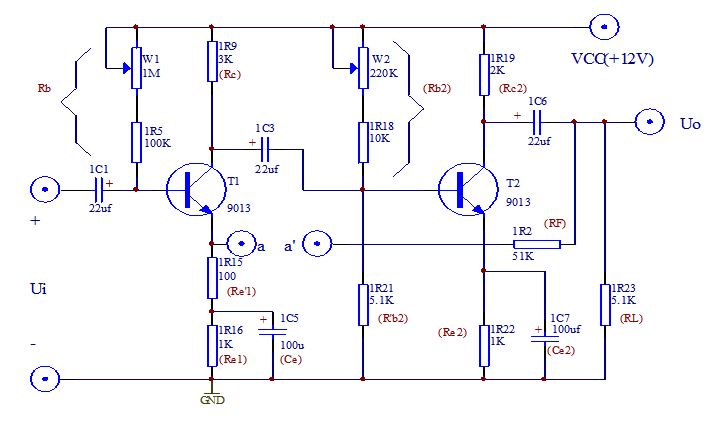
\includegraphics[width=0.4\linewidth]{电路图2.png}
		\caption{实验电路图}
		\label{}
	\end{figure}
	实验电路图如上图所示,是一个串联电压负反馈放大电路。该电路输出电压$U_0$通过电阻$R_f$和$R_{e1}$分压后送回到第一级放大电路的输入回路,从而引入交流电压串联负反馈。电压负反馈的重要特点是电路的输出电压趋于稳定,因为无论反馈信号以何种方式引回到输入端,实际上都是利用输出电压$U_0$本身通过反馈网络对放大电路起自动调整作用。若当$U_i$一定时,若负载电阻$R_L$减小而使输出电压$U_0$下降,则电路将进行如下的自动调整过程:
	$$R_{L}\downarrow-\rightarrow U_{o}\downarrow-\rightarrow U_{f}\downarrow-\rightarrow U_{be}\uparrow-\rightarrow U_{o}\uparrow $$

	 (1) 负反馈降低了放大器的电压放大倍数
$$A_{u}=\frac{U_{o}}{U_{i}}\\F=\frac{R_{e1}}{R_{e1}+R_{f}}$$
$$U_{f}=FU_{o}$$
$$A_{uf}=\frac{A_{u}}{1+A_{u}F}$$

(2)负反馈提高了放大器放大倍数的稳定性
$$\frac{\Delta A_{uf}}{A_{uf}}=\frac{\Delta A_{u}}{A_{u}}\frac{1}{1+A_{u}F}$$

 (3) 负反馈展宽了放大器的频带
	\begin{figure}[{H}]
		\centering
		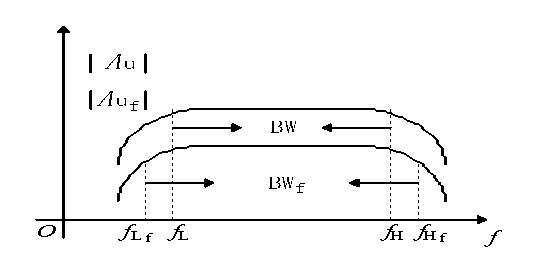
\includegraphics[width=0.4\linewidth]{频宽放大.png}
		\caption{频带加宽}
		\label{}
	\end{figure}
	
	
	
	
	% 实验记录	
	\clearpage
	
	% 顶栏
	\begin{table}
		\renewcommand\arraystretch{1.7}
		\centering
		\begin{tabularx}{\textwidth}{|X|X|X|X|}
			\hline
			专业: & 物理学 & 年级: & 2022级 \\
			\hline
			姓名: & 黄罗琳、王显 & 学号: &22344001、22344002 \\
			\hline
			室温: &23℃  & 实验地点: & A522 \\
			\hline
			学生签名:&  & 评分: &\\
			\hline
			实验时间:& 2024/5/8 & 教师签名:&\\
			\hline
		\end{tabularx}
	\end{table}
	% ---
	
	% 小标题
	\section{ET9两级阻容耦合放大电路 \quad\heiti 实验记录}
	% ---
	
	% 实验过程记录
	\subsection{调整静态工作点}
	首先将电源电压调到 $V_{cc}=12V$,调节电位器 $R_{W1}$,使
$U_{C1}=9-10V$,调节电位器 $R_{W2}$,使$U_{C2}=6-7$V。给放大器输入一个频率为
$1KHZ$,大小为 2mV 的信号。用示波器分别观察第一级和第二级放大器输出波形。若波形有失真,则可微调 W1、W2,直到使两级放大器输出信号波形都不失真为止。测量晶体管 $T_1$与 $T_2$的各极电位。
	\begin{figure}[{H}]
		\centering
		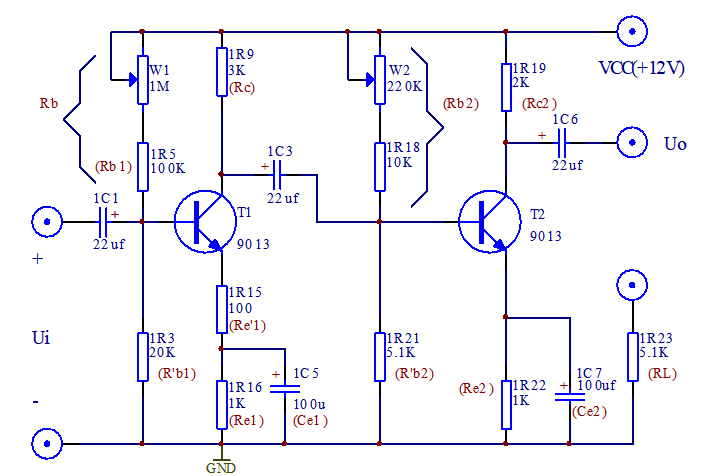
\includegraphics[width=0.4\linewidth]{电路图1.png}
		\caption{实验电路图}
		\label{}
	\end{figure}
	\begin{figure}[{H}]
		\centering
		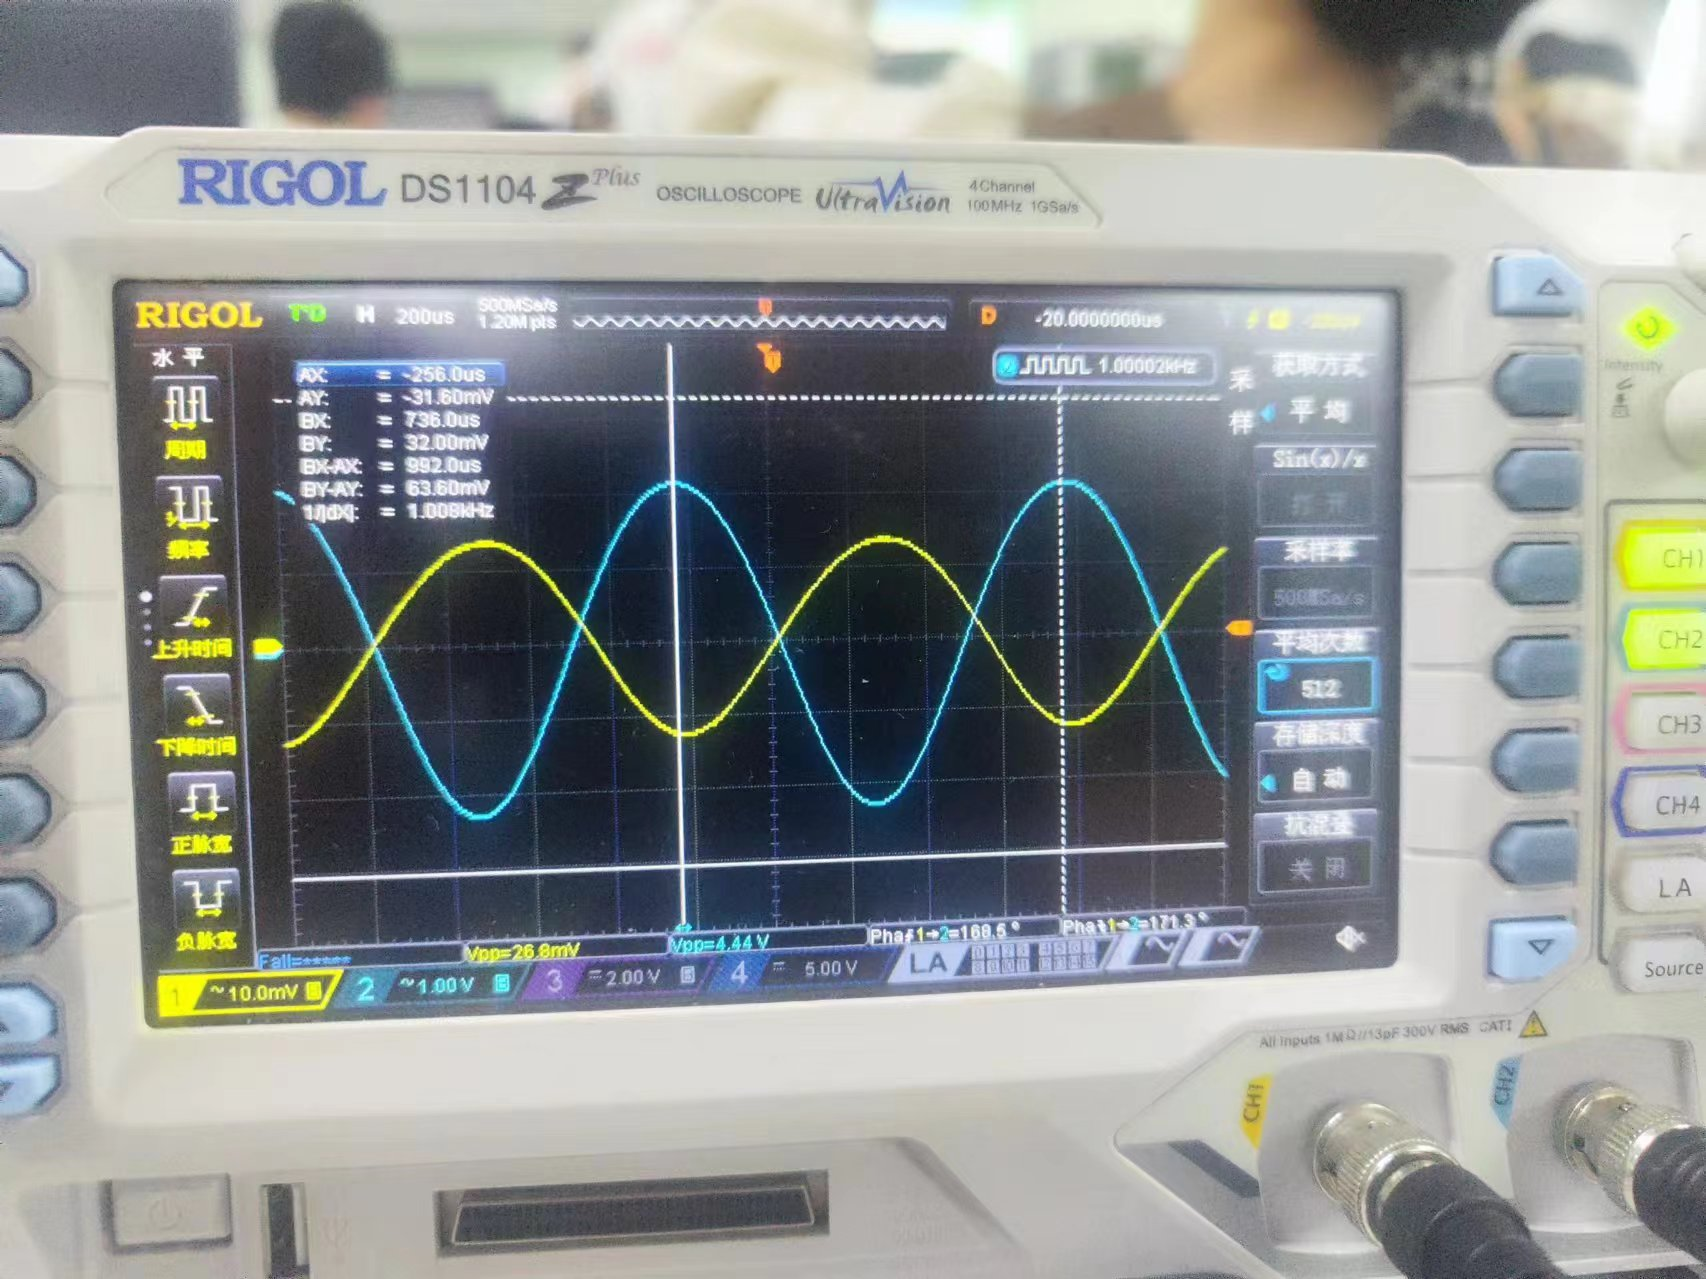
\includegraphics[width=0.4\linewidth]{不失真.jpg}
		\caption{示波器图像}
		\label{}
	\end{figure}
	\begin{table}[h]
		\centering
		\caption{实验数据}
	\begin{tabular}{|c|c|c|c|c|c|}
	
		\hline
		  \multicolumn{3}{|c|}{\textbf{T1 相线}} & \multicolumn{3}{|c|}{\textbf{T2 相线}}\\
		\hline
		\textbf{Ucl (V)} & \textbf{Ub1 (V)} & \textbf{Ue1 (V)} & \textbf{Uc2 (V)} & \textbf{Ub2 (V)}&  \textbf{Ue2 (V)}\\
		\hline
		9.577&1.737 &1.124 &6.564 &2.902 &2.267\\
		\hline
		\end{tabular}
	\end{table}
	\subsection{测量电压放大倍数}
	输入信号仍为f=lKHz、2mV交流信号,在不失真的情况下,按给定的条件,分别测量放大器的第一级和第二级的输出电压$U_{01}$,$U_0$。
	\begin{table}[ht]
		\centering
		\caption{实验数据}
		\begin{tabular}{|c|c|c|c|c|c|c|c|}
			\hline
			\multirow{2}{*}{条件} & \multicolumn{3}{c|}{测量输入与输出电压} & \multicolumn{3}{c|}{计算电压放大倍数}\\
			\cline{2-7}
			 & Ui (V) & Uo1 (V) & Uo (V)& $ A_{u1} = \frac{U_{o1}}{U_i}$ &$ A_{u2} = \frac{U_o}{U_{o1}}$ & $A_u = \frac{U_o}{U_i}$\\
			\hline
			
			\hline
			 $R_L=\infty$ &1.381mv&9.257mv &1.664V&6.712&179.756&1204.924\\
			\hline
			 $R_L=5.1K\Omega $&1.380mV&9.313mV&1.146V&6.748&123.054 &830.435\\
			\hline
		\end{tabular}
		
		
		\end{table}
		\subsection{用逐点测量法测试放大器幅频特性}
		\begin{enumerate}
			\item 保持输入信号$U_i=2mV$不变,接入负载$R_L=5.1K\Omega$,改变频率测出相应的输出电压$U_0$。
			\item 找出上下限截止频率$f_H$,$f_L$(增益下降到中频增益的0.707倍时所对应的频率点,即3分贝点),并求出放大器的带宽,$B_W=f_H—f_L$
		\end{enumerate}
	



		\begin{table}[h]
			\centering
			\caption{实验数据}
			\begin{tabular}{|c|*{12}{c|}}
				\hline
				$f(HZ)$ & 10 & 20 & 30 & 40 & 50 & 60 & 70 & 80.8 & 90 & 100 & 120 & 150 \\
				\hline
				$U_0(V)$ & 0.086 & 0.232 & 0.373 & 0.494 & 0.596 & 0.678 & 0.745 & 0.810 & 0.851 & 0.888 & 0.947 & 1.009 \\
				\hline
				$Au$ & 43.0 & 116.0 & 186.5 & 247.0 & 298.0 & 339.0 & 372.5 & 405.0 & 425.5 & 444.0 & 473.5 & 504.5 \\
				\hline
				$f(HZ)$ & 200 & 300 & 500 & 800 & 1000 & 1200 & 1400 & 2200 & 3000 & 3800 & 5000 & 6000 \\
				\hline
				$U_0(V)$ & 1.051 & 1.098 & 1.128 & 1.134 & 1.134 & 1.131 & 1.126 & 1.096 & 1.056 & 1.009 & 0.937 & 0.880 \\
				\hline
				$Au$ & 525.5 & 549.0 & 564.0 & 567.0 & 567.0 & 565.5 & 563.0 & 548.0 & 528.0 & 504.5 & 468.5 & 440.0 \\
				\hline
				$f(HZ)$ & 6500 & 7200 & 7500 & 8000 & 10k & 15k & 20k & 30k & 40k & 50k & 100k & \\
				\hline
				$U_0(V)$ & 0.849 & 0.810 & 0.792 & 0.765 & 0.671 & 0.498 & 0.391 & 0.267 & 0.201 & 0.160 & 0.073 & \\
				\hline
				$Au$ & 424.5 & 405.0 & 396.0 & 382.5 & 335.5 & 249.0 & 195.5 & 133.5 & 100.5 & 80.0 & 36.5 & \\
				\hline
			\end{tabular}
		\end{table}

	% ---
	
	
	
	% 分析与讨论	
	\clearpage
	% 顶栏
	\begin{table}
		\renewcommand\arraystretch{1.7}
		\centering
		\begin{tabularx}{\textwidth}{|X|X|X|X|}
			\hline
			专业: & 物理学 & 年级: & 2022级 \\
			\hline
			姓名: & 黄罗琳、王显 & 学号: &22344001、22344002 \\
			\hline
			室温: &23℃  & 实验地点: & A522 \\
			\hline
			学生签名:& 
\includegraphics[width=1cm]{签字.jpg} 
\includegraphics[width=1cm]{wx.jpg} & 评分: &\\
			\hline
			实验时间:& 2024/5/15 & 教师签名:&\\
			\hline
		\end{tabularx}
	\end{table}
	\section{ET10负反馈放大电路 \quad\heiti 实验记录}
	
\subsection{调整静态工作点}
	电路如图所示,连接$a$,$a'$点使放大器处于闭环工作状态。输入端对地短路($U_i=0$),经检查无误后,方可接通电源,调整$W1$、$W2$使$I_{C1}=I_{C2}=2mA$时,测量各级静态工作点。
	\begin{figure}[H]
		\centering
		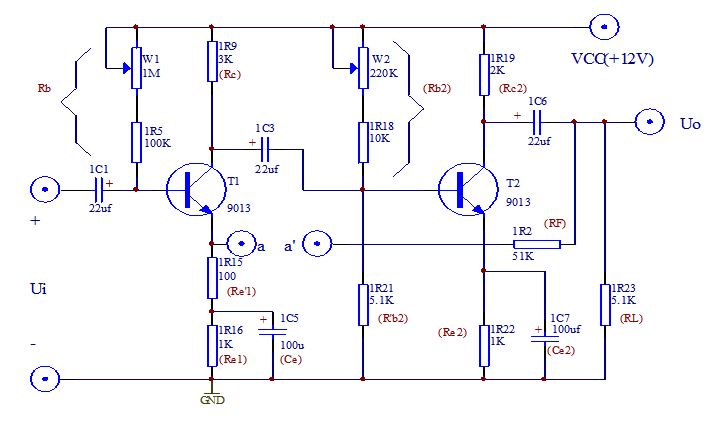
\includegraphics[width=0.4\linewidth]{电路图2.png}
		\caption{实验电路图}
		\label{}
	\end{figure}
	\begin{table}[H]
		\centering
		\begin{tabular}{|c|c|c|c|c|c|c|}
			\hline
			待测参数 & $UC1$(V) & $UB1$(V) & $UE1$(V) & $UC2(V)$ &$ UB2$(V) & $UE2$(V) \\
			\hline
			测量值 &7.156 &2.815 & 2.187& 7.714& 2.648&2.017 \\
			\hline
		\end{tabular}
	
		\end{table}
		\subsection{观察负反馈对放大倍数的影响}
		在输入端加入$U_i=2$mV$,f=1$kHz的正弦信号,分别测量电路在开环与闭环工作时的输出电压$U_{0}$,同时用示波器观察输出波形,此时波形不失真,计算电路在开环与闭环工作时的电压放大倍数,记入下表中。


		\begin{table}[H]
			\centering
			\begin{tabular}{|c|c|c|}
				\hline
				工作方式 & UO(V) & Au或Auf \\
			
			
				\hline
				开环 & 1.158& 818.83\\
				\hline
				闭环 & 0.10085&71.31 \\
				\hline
			\end{tabular}
			\end{table}
			\subsection{观察负反馈对放大倍数稳定性的影响}
			当改变电源电压$V_{cc}$从12V变到10V,并在输入端加入$2mV$、$1kHz$的正弦波信号时,分别测量电路在开环和闭环工作状态时的输出电压。在这种情况下,确保波形不失真。接着,计算电路在开环和闭环工作时的电压放大倍数,并将结果记录在下表中。
			\begin{table}[H]
				\centering
				\begin{tabular}{|c|c|c|c|c|}
					\hline
					\multirow{2}{*}{测量参数} & \multicolumn{2}{c|}{VCC = 12V} & \multicolumn{2}{c|}{VCC = 10V} \\
					\cline{2-5}
					 & UO(V) & Au或Auf & UO(V) & Au或Auf \\
					\hline
					开环 & 1.158&818.83 &0.985 & 696.50\\
					\hline
					闭环 & 100.85mv&71.31 &99.19mv &70.14 \\
					\hline
				\end{tabular}
			
				\end{table}
				\subsection{幅频特性测量}
				Vcc=12V(不接负载),在输入端加入 U$_\mathrm{i}=2$mV,f=1KHz 的正弦波信号,然后调节信号源频率使 f 下降(保持 Ui 不变)测量 Uo,且在电压放大倍数下降到中频电压放大倍数的0.707倍时所对应的频率点附近时,多测几点,找出下限频率,同理使 f 上升,找出上限频率,求出放大器的带宽$BW{=}f_{\mathrm{H}}{—}f_{\mathrm{L}}{。}$,并对开环、闭环状态进行比较。
				\begin{enumerate}
					\item 开环 
					\begin{table}[H]
						\centering
						\begin{tabular}{|c|*{12}{c|}}
							\hline
							$f(HZ)$ & 10 & 20 & 25 & 30 & 40 & 45 & 50 & 60 & 77.5 & 100 & 130 & 150 \\
							\hline
							$U_0(V)$ & 90.56 & 244 & 321 & 394 & 522 & 578 & 633 & 711 & 819 & 919 & 992 & 1024 \\
							\hline
							$f(HZ)$ & 200 & 500 & 1000 & 2000 & 3000 & 4000 & 5000 & 6000 & 7000 & 8000 & 9000 & 10000 \\
							\hline
							$U_0(V)$ & 1074 & 1145 & 1157 & 1148 & 1128 & 1103 & 1075 & 1041 & 1007 & 971 & 934 & 897 \\
							\hline
							$f(HZ)$ & 12200 & 14000 & 16000 & 18000 & 20000 & 21200 & 22000 & 25000 & 30000 & 40000 & & \\
							\hline
							$U_0(V)$ & 819 & 763 & 704 & 651 & 606 & 578 & 563 & 508 & 435 & 332 & & \\
							\hline
						\end{tabular}
					\end{table}
					
				\item 闭环
				\begin{table}[H]
					\centering
					\begin{tabular}{|c|*{10}{c|}c|}
						\hline
						$f(HZ)$ & 10 & 12 & 15 & 20 & 23 & 30 & 40 & 50 & 70 & 100 \\
						\hline
						$U_0(V)$ & 36.75 & 44.61 & 54.24 & 66.02 & 71.3 & 79.96 & 86.79 & 90.93 & 94.82 & 97.96 \\
						\hline
						$f(HZ)$ & 200 & 500 & 1000 & 2000 & 5000 & 10000 & 20000 & 50000 & 80000 & 90000 \\
						\hline
						$U_0(V)$ & 99.74 & 100.73 & 100.89 & 100.99 & 101.15 & 101.23 & 101.51 & 102.45 & 101.79 & 100.4 \\
						\hline
						$f(HZ)$ & 100000 & 110000 & 120000 & 130000 & 140000 & 150000 & 159000 & 170000 & 180000 & 200000 \\
						\hline
						$U_0(V)$ & 98 & 96.9 & 92.62 & 87.73 & 82.28 & 76.56 & 71.3 & 65.26 & 59.84 & 50.27 \\
						\hline
					\end{tabular}
				\end{table}
				
				
				\end{enumerate}
				\subsection{用示波器观察负反馈对放大器非线性失真的改善}
				\begin{figure}[{H}]
		\centering
		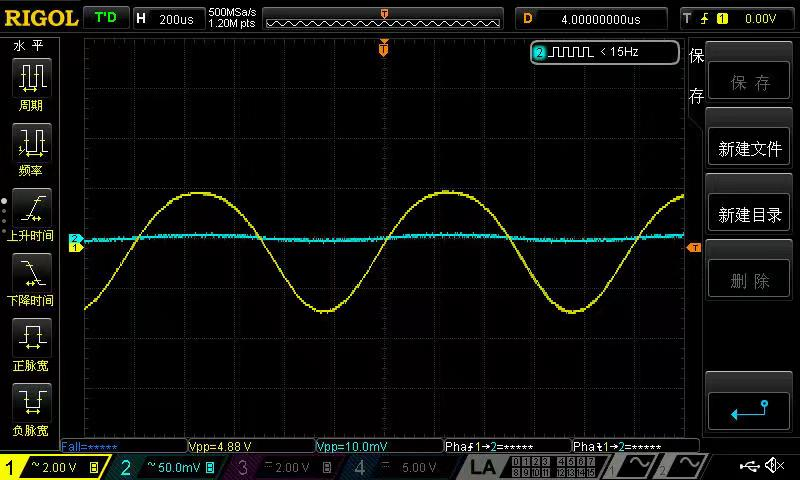
\includegraphics[width=0.8\linewidth]{改善1.jpg}
		\label{}
	\end{figure}
	\begin{figure}[{H}]
		\centering
		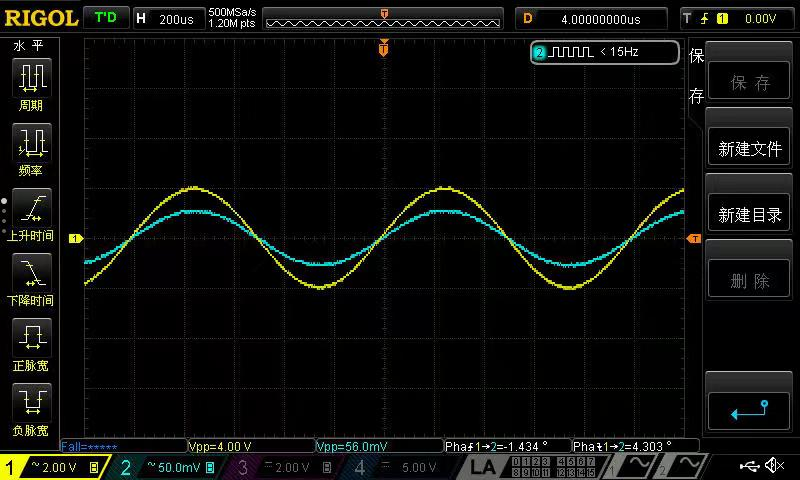
\includegraphics[width=0.8\linewidth]{改善2.jpg}
		\label{}
	\end{figure}

\clearpage
	% 顶栏
	\begin{table}
		\renewcommand\arraystretch{1.7}
		\begin{tabularx}{\textwidth}{|X|X|X|X|}
			\hline
			专业:& 物理学 &年级:& 2022级\\
			\hline
			姓名: &黄罗琳 、王显 & 学号:&22344001、22344002 \\
			\hline
			日期:& 2024/5/8  & 评分: &\\
			\hline
		\end{tabularx}
	\end{table}
	% ---
	
	% 小标题
	\section{ET9两级阻容耦合放大电路 \quad\heiti 分析与讨论}
	

	
	%
	\subsection{对于测量电压放大倍数的讨论}
	输入信号仍为$f=lKHZ$\quad $2mV$交流信号,在不失真的情况下,按给定的条件,分别测量放大器的第一级和第二级的输出电压$U_{01}$,$U_0$。
	\begin{table}[ht]
		\centering
		\caption{理论值、实验值及相对误差}
		\begin{tabular}{|c|c|c|c|}
		\hline
		条件 & 理论值 ($A_{u1} \times A_{u2}$) & 实验值 ($A_u$) & 相对误差 \% \\
		\hline
		$R_L=\infty$ & 1206.44 & 1204.924 & 0.126 \\
		\hline
		$R_L=5.1K\Omega$ & 830.37 & 830.435 & 0.008 \\
		\hline
		\end{tabular}
		\end{table}
		\begin{enumerate}
			\item 验证放大倍数的乘积关系
			
			从数据来看,理论值与实验值的相对误差非常小,分别为0.126\%和0.008\%。这表明实验结果很好地验证了总的放大倍数等于各级放大倍数的乘积,即$A_u = A_{u1} \times A_{u2}$。实验值与理论值的极小差异验证了放大电路设计的准确性,证明了在理想条件下总放大倍数等于各级放大倍数的乘积。
			\item 负载电阻对放大倍数的影响
			
			当负载电阻$R_L$从无穷大变为5.1kΩ时,总放大倍数明显降低,从1204.924降至830.435。放大倍数的降低可以归因于负载效应。当负载电阻接入电路后,输出电压被分担,导致放大倍数下降。这种现象在实际电路中常见,是因为负载电阻影响了输出电压的分布。
		\end{enumerate}
		
	%
	\subsection{ 用逐点测量法测试放大器幅频特性}
	\begin{figure}[{H}]
		\centering
		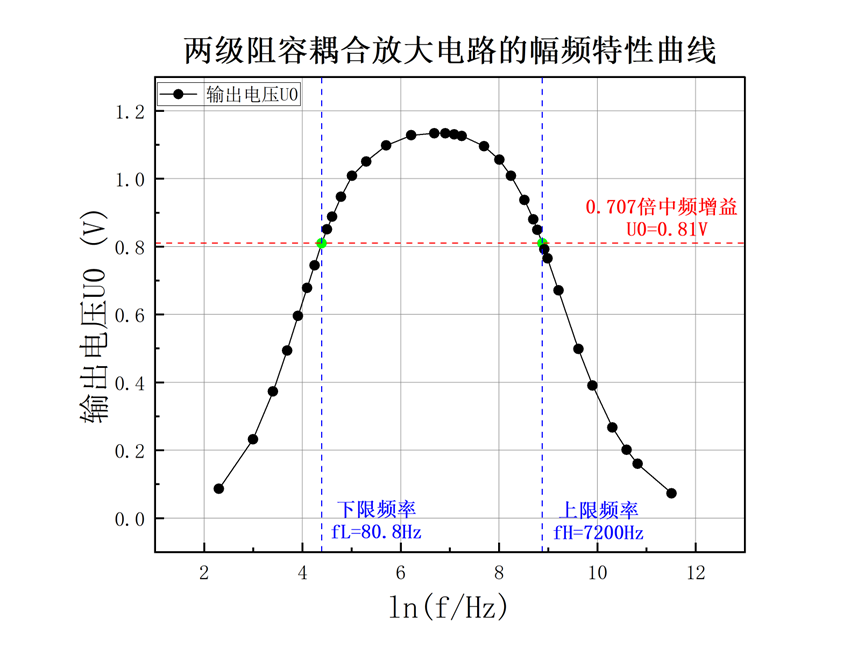
\includegraphics[width=0.8\linewidth]{幅频.png}
		\label{}
	\end{figure}
	由实验数据及图像可知,$f_H=7200$Hz,$f_L=80.8$Hz
	带宽$B_W=f_H-f_{L}=7119.2Hz$.
	%

	
	% ---
	
	% 实验后思考题
	\subsection{实验思考题}
	
	%思考题1
	\begin{question}
		如何增加阻容耦合放大器的频率范围?
	\end{question}
	增加阻容耦合放大器的频率范围可以通过多种方法实现。阻容耦合放大器的频率范围通常受到以下因素的限制:放大器的带宽、截止频率、稳定性等。
	\begin{enumerate}
	
	
	

	\item 增加带宽限制器的频宽:选择更高频率的放大器和其他组件可以增加阻容耦合放大器的频率范围。例如,选择高速运算放大器或高频率的二极管、电容器等。

	\item 减小输入和输出的电容值:输入和输出的电容值会影响放大器的频率响应。通过减小输入和输出电容的数值,可以增加阻容耦合放大器的频率范围。但是,这也可能会导致增加噪声和降低稳定性,需要在设计中做出权衡。

	\item 选择高品质的被动元件:选择具有更高频率响应的被动元件,例如高频率响应的电容器和电阻器,可以增加阻容耦合放大器的频率范围。

	\item 优化反馈网络:调整反馈网络的参数,如增益和带宽积,可以改善放大器的频率响应。合适的反馈网络设计可以提高放大器的带宽和稳定性。
	
\end{enumerate}

	% ---
	
	
	% 结语部分
	\clearpage
	\begin{table}
		\renewcommand\arraystretch{1.7}
		\begin{tabularx}{\textwidth}{|X|X|X|X|}
			\hline
			专业:& 物理学 &年级:& 2022级\\
			\hline
			姓名: &黄罗琳 、王显 & 学号:&22344001、22344002 \\
			\hline
			日期:& 2024/5/15  & 评分: &\\
			\hline
		\end{tabularx}
	\end{table}
	\section{ET10负反馈放大电路 \quad\heiti 分析与讨论}
	
	\subsection{实验数据绘图}
	\begin{figure}[{H}]
		\centering
		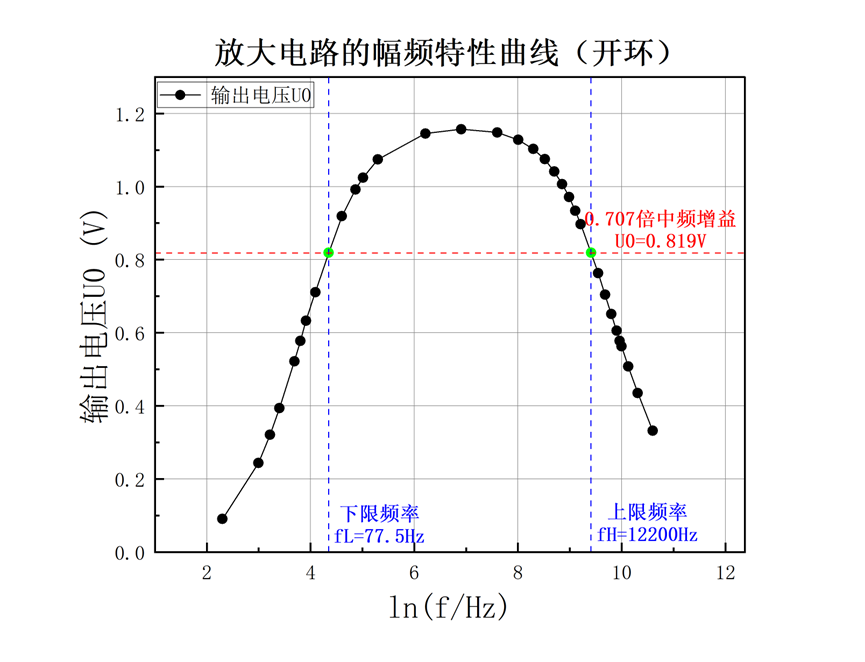
\includegraphics[width=0.6\linewidth]{开环.png}
		
		\label{}
	\end{figure}
	
	\begin{figure}[{H}]
		\centering
		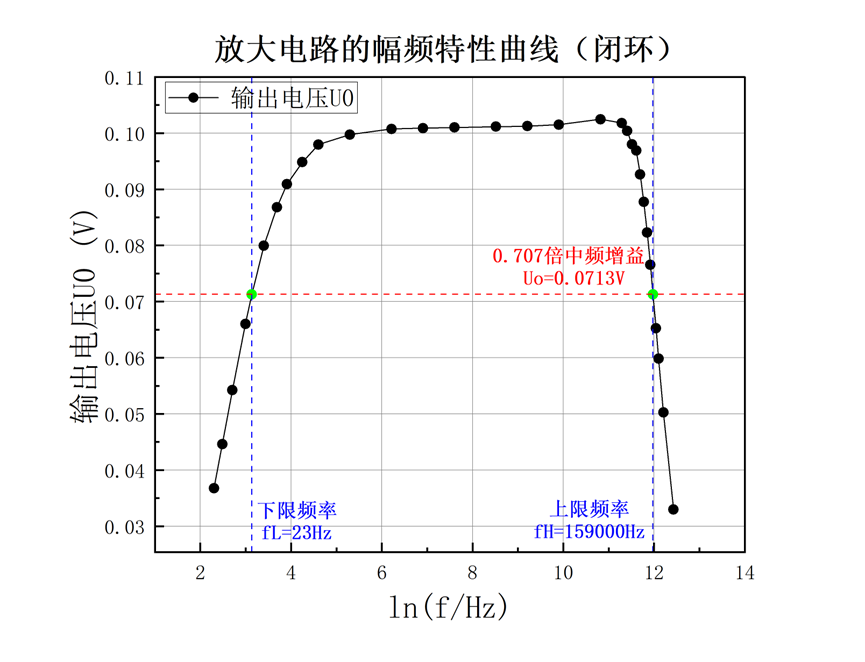
\includegraphics[width=0.6\linewidth]{闭环.png}
		
		\label{}
	\end{figure}
	\subsection{实验数据分析}
	开环 $B_W=12200-77.5=12122.5Hz$

闭环$B_W=159000-23=158977Hz$

\textbf{闭环状态的上限频率更高、下限频率更低,带宽更大。
}

在开环状态下,放大器的增益很高,这意味着即使输入信号很小,输出信号也会经过放大器的放大,从而可能导致失真。因为放大器的增益高,它对输入信号的变化非常敏感。一旦输入信号达到某个水平,放大器就可能开始饱和,导致输出信号失真。

然而,在负反馈放大器中,一旦负反馈被应用,系统的整体增益会下降。这意味着相同的输入信号在输出端产生的信号幅度会变小。因此,在负反馈作用下,输入信号需要更大的振幅才能使输出信号饱和,因为放大器的整体增益已经被降低了。

具体来说,负反馈放大器中的负反馈会将一部分输出信号反馈到输入端,并与输入信号相减,从而减小放大器的总增益。这样,即使输入信号增加到会导致开环放大器饱和的水平,负反馈也会减小输出信号,使其在正常范围内保持线性,而不至于失真。

因此,负反馈放大器在闭环状态下对输入信号的容纳能力更强,可以处理更大振幅的输入信号而不至于失真,这是因为负反馈降低了系统的增益。这就是为什么在闭环状态下,放大器的最大不失真电压远大于开环状态的原因。

\subsection{实验思考题}
	
	%思考题1
	\begin{question}
		本实验电路中引入了哪些反馈?分析它们的组态和对放大器性能的影响。
	\end{question}
	在电路中,引入了电压负反馈。具体来说,是串联电压负反馈。
负反馈信号是通过输出电压$U_0$分压后送回到第一级放大电路的输入回路。这种负反馈通过电阻$R_f$和$R_{e1}$形成,构成了一个反馈网络,将一部分输出电压作为反馈信号送回到输入端。

稳定性提高:通过降低电路的电压放大倍数,负反馈使得放大器的输出电压更加稳定。即使负载电阻$R_L$发生变化,输出电压$U_0$也会被调整以使得输入信号$U_i$和反馈信号$U_f$之间的比值保持稳定。

带宽增加:通常负反馈可以增加放大器的带宽,因为它降低了放大器的增益,使得放大器的频率响应更平坦。

谐波失真减小:负反馈可以减小放大器的谐波失真,使得输出信号更接近输入信号的形状。
输入/输出阻抗影响:负反馈可以降低放大器的输入和输出阻抗,使得放大器更容易驱动负载并更容易与外部电路匹配。

总的来说,负反馈可以改善放大器的线性度、稳定性和频率响应,从而提高整体性能。
\begin{question}
	负反馈放大电路的开环等效电路的画法规则是什么?
\end{question}

断开反馈环路:在适当的位置断开反馈网络,确保能测量到开环增益。

添加信号源:在断开点处添加一个测试信号源,用于模拟输入信号。

保留原电路的其余部分:保留原电路中的所有其他元件,包括放大器和任何无反馈的连接元件。

\clearpage
	\section{ ET9、ET10 两级阻容耦合放大电路、负反馈放大电路 \quad\heiti 结语}
	% ---
	
	% 总结、杂谈与致谢
	\subsection{实验心得和体会、意见建议等}
	\begin{enumerate}
		\item 两个实验总体接线难度较大,需要足够的细心和耐心,可能有些错误的接线会导致实验数据的错误。这种错误往往需要与其他小组进行相互验证才能发现。
		\item 实验需要各小组之间的配合与讨论,实验较长时间处于debug阶段。
		\item \textbf{本实验报告采用LATEX编辑,实验分工为黄罗琳同学负责记录数据、编辑报告、数据分析,王显同学负责实验操作、误差分析、数据绘图。}
	\end{enumerate}
	\quad \large \textbf{感谢您对于此篇实验报告的阅读与批改,祝您工作顺利!}
	% ---
	

	% 附件
	\subsection{附件}
	\begin{figure}[H]
		\centering
		\begin{minipage}{0.3\textwidth}
			\centering
			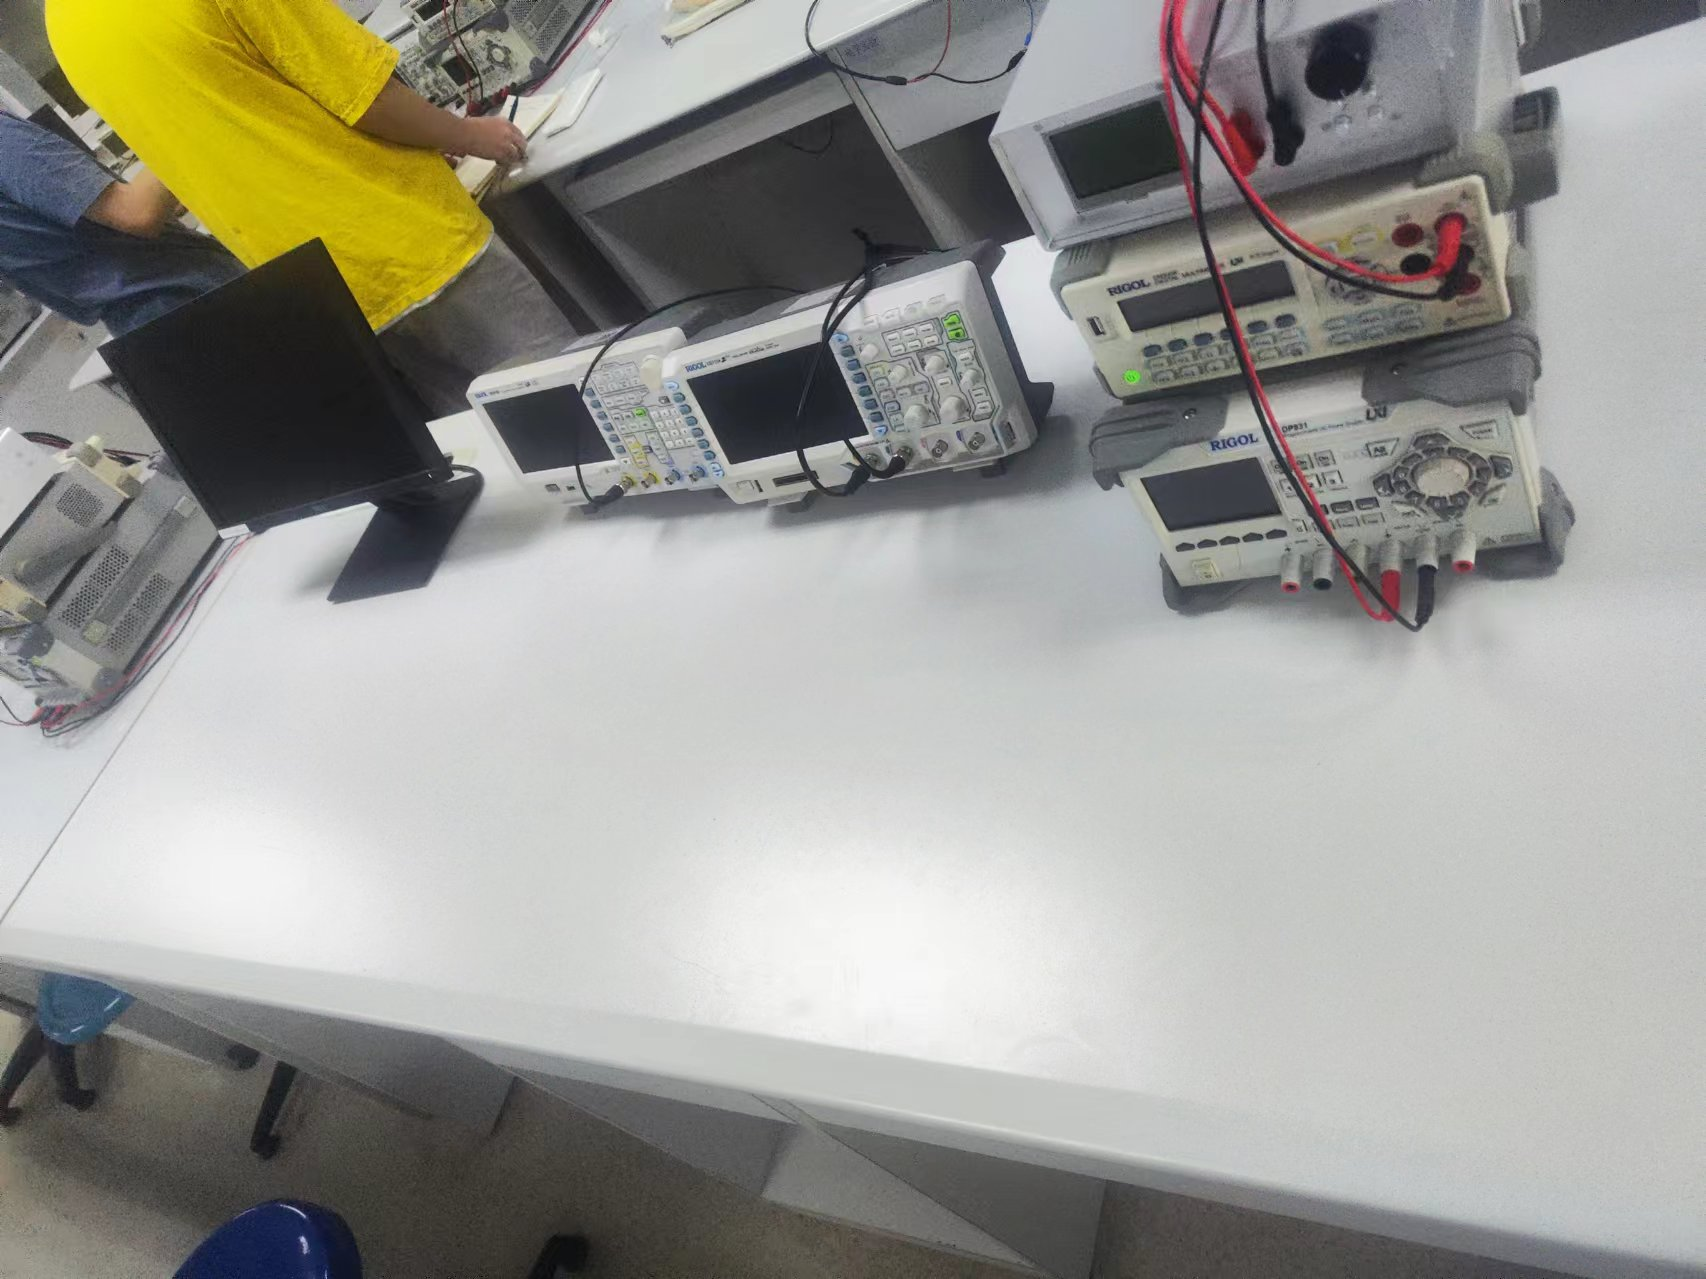
\includegraphics[width=\linewidth]{桌面.jpg}
			\caption{桌面}
		\end{minipage}\hfill
		\begin{minipage}{0.3\textwidth}
			\centering
			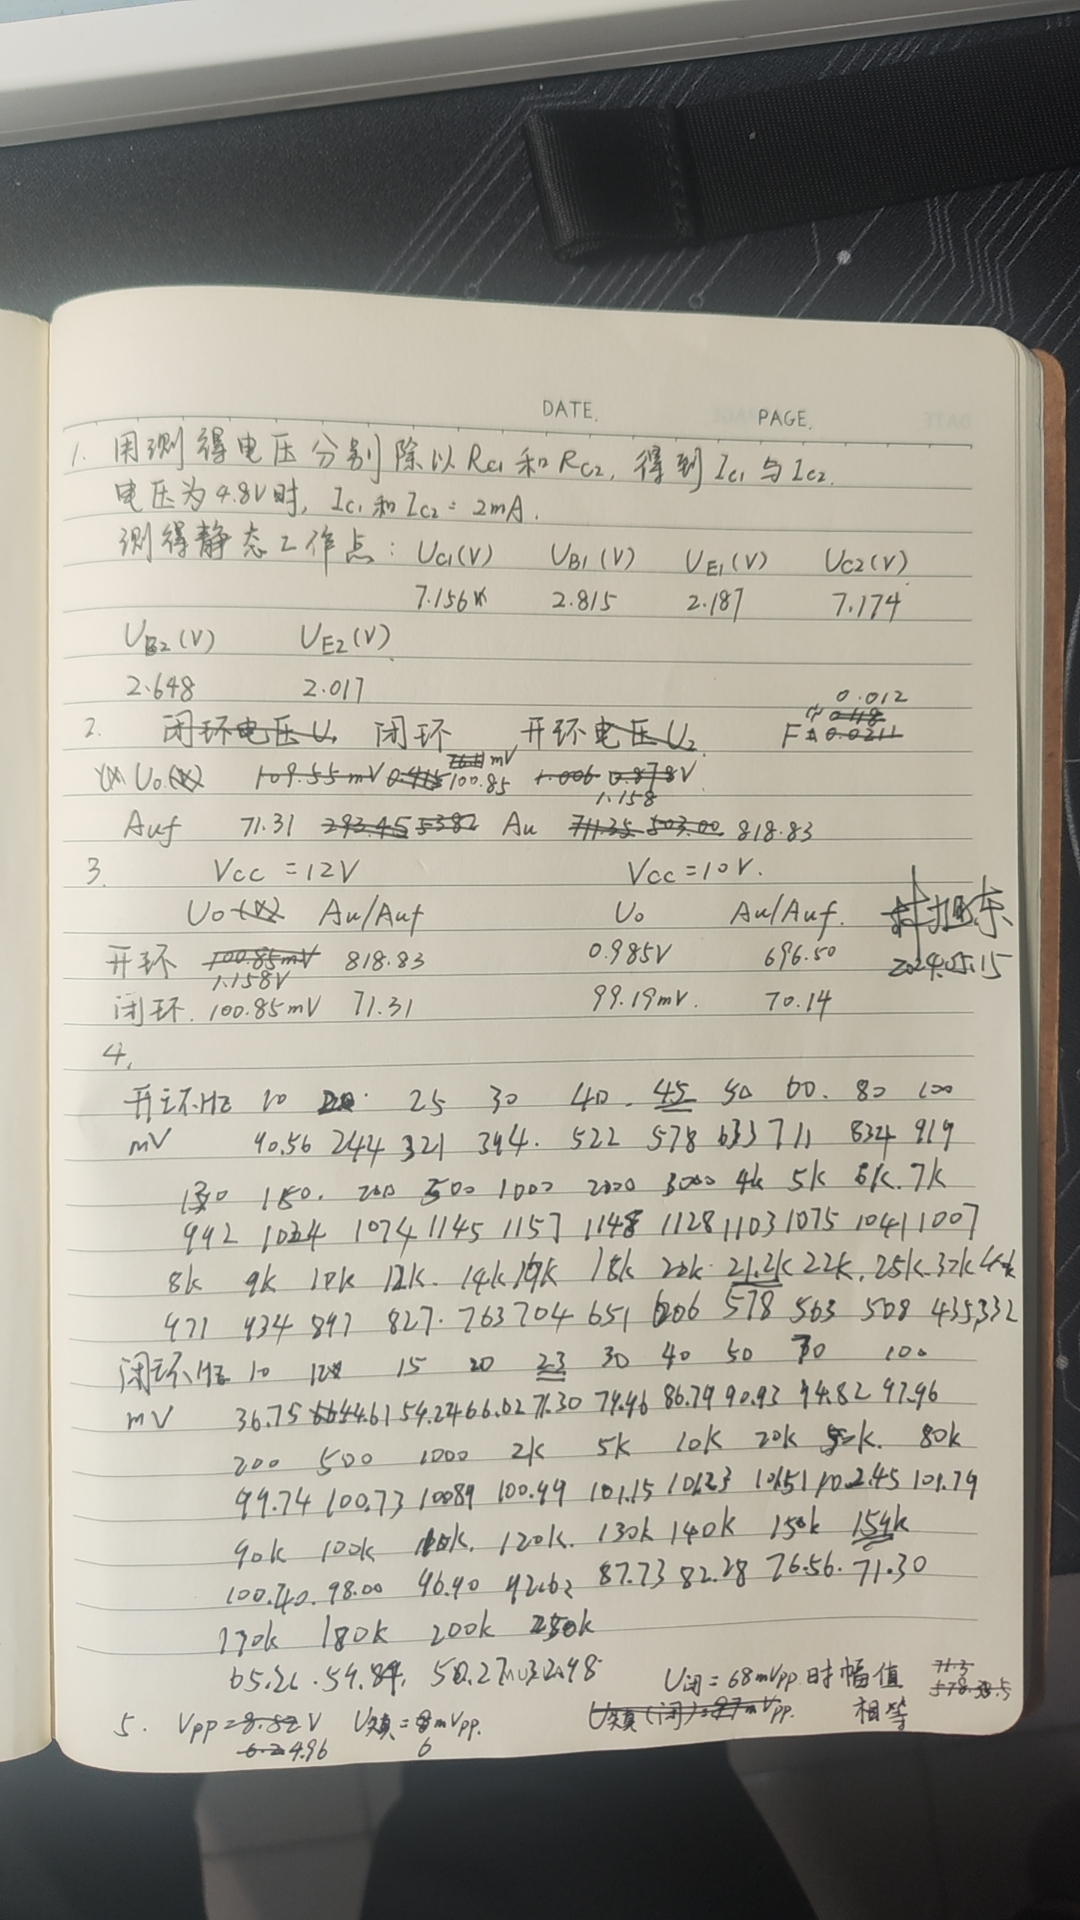
\includegraphics[width=\linewidth]{原始数据.jpg}
			\caption{原始数据}
		\end{minipage}\hfill
		\begin{minipage}{0.3\textwidth}
			\centering
			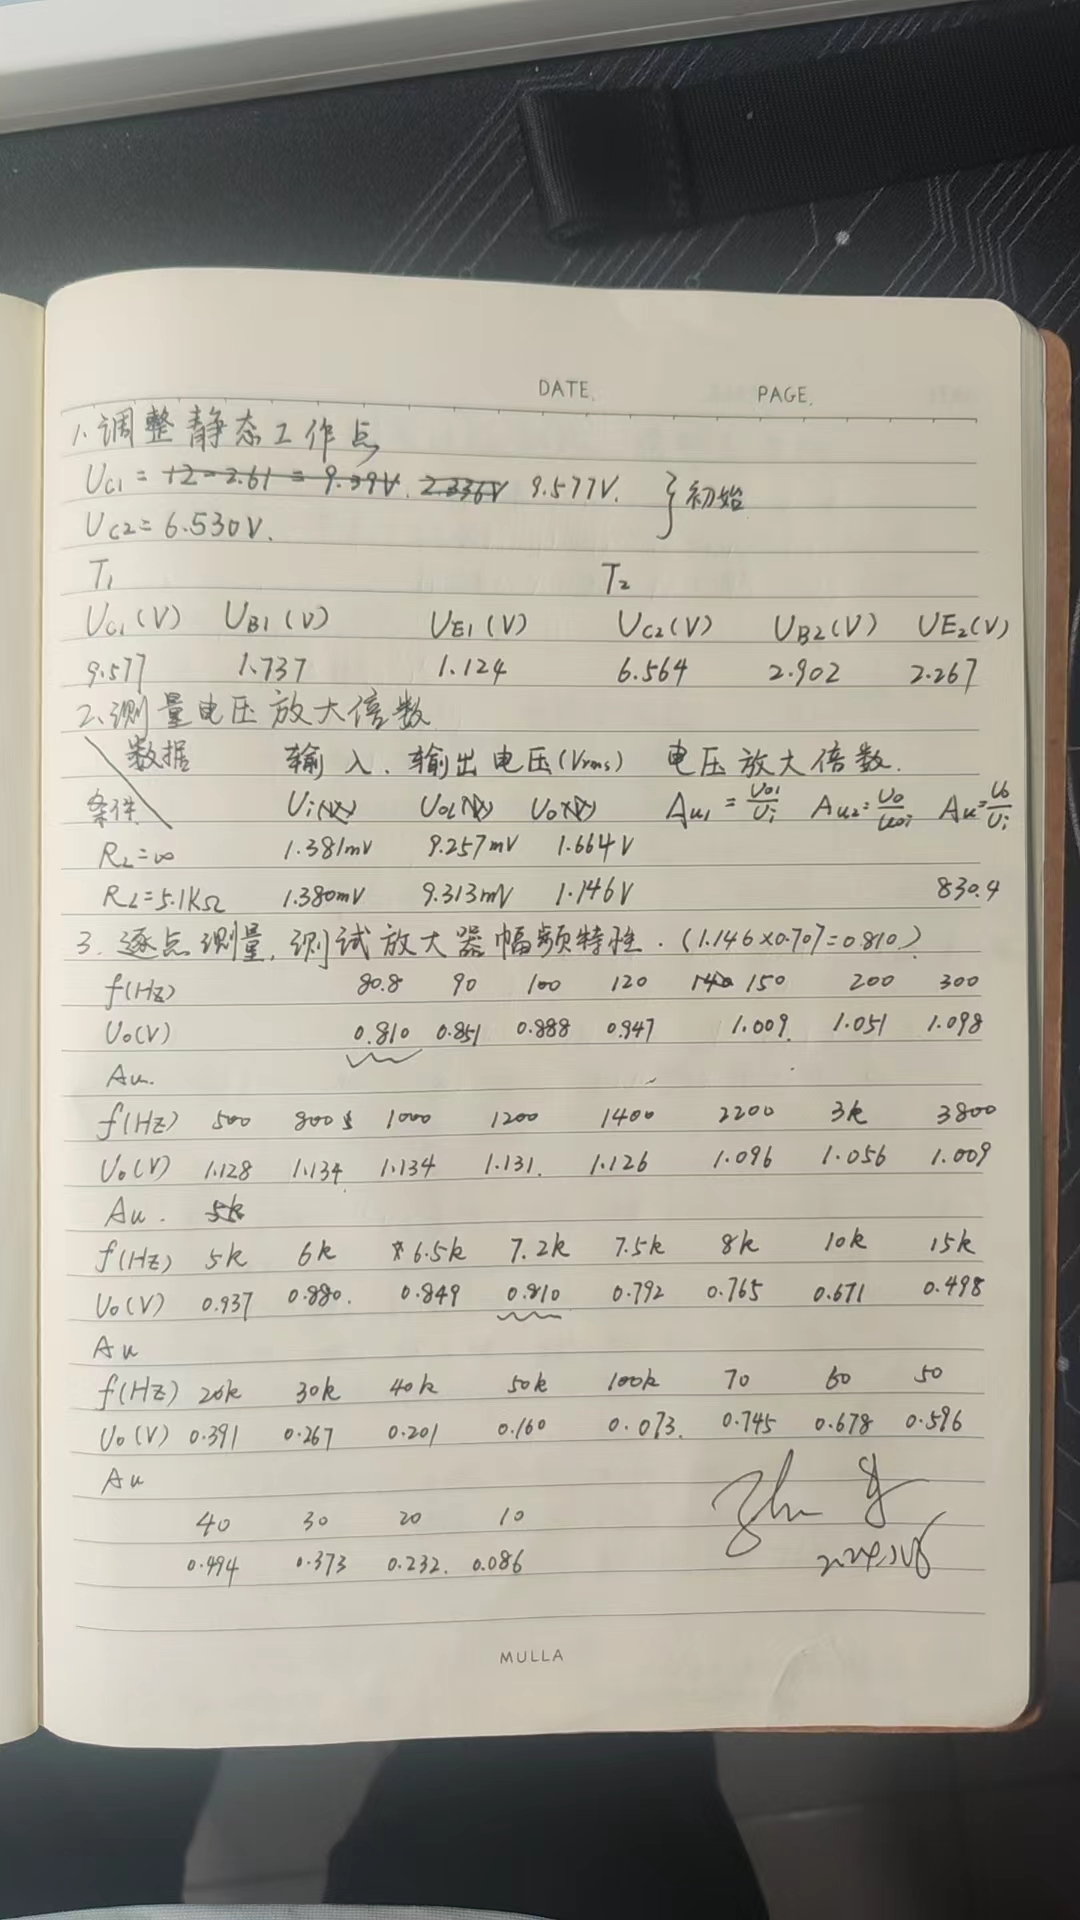
\includegraphics[width=\linewidth]{原始数据1.jpg}
			\caption{原始数据}
		\end{minipage}
	\end{figure}
	% ---
	
	
\end{document}